% !TEX ROOT = ../ersti.tex
\section{Vorkurs Physik}
Der Vorkurs Physik besteht aus einem mathematischen Vorkurs der Fakultät für Physik und Astronomie, gelesen von \dozentvorkurs. Dieser gehört zum Curriculum, ist aber nicht verpflichtend. Dennoch: ihr könnt hier bereits durch den Vorkurs eure ersten Credit-Points erhalten! Er beginnt am 25. September um 9 Uhr und findet vor Ort statt. Die genauen Inhalte des Vorkurses legen die Dozenten je nach Kenntnisstand der Hörerschaft fest, wobei das zugehörige Skript\footnote{\url{https://www.thphys.uni-heidelberg.de/~hefft/vk3/}} einen guten Anhaltspunkt bietet. Einen genauen Plan der Vorkursveranstaltungen und Orte findet ihr im Internet\footnote{\url{http://mathphys.info/vorkurs/plan\#physik}}.

% Den Vorkurs gibt es inzwischen auch als gebundenes Buch (siehe Buchliste). Geht ruhig mal in der ersten Vorkurswoche in die Universitätsbibliothek und leiht es euch sozusagen als Begleitbuch aus. (Vom Kauf möchten wir dennoch abraten.)

\begin{figure*}[!b]
    \centering
    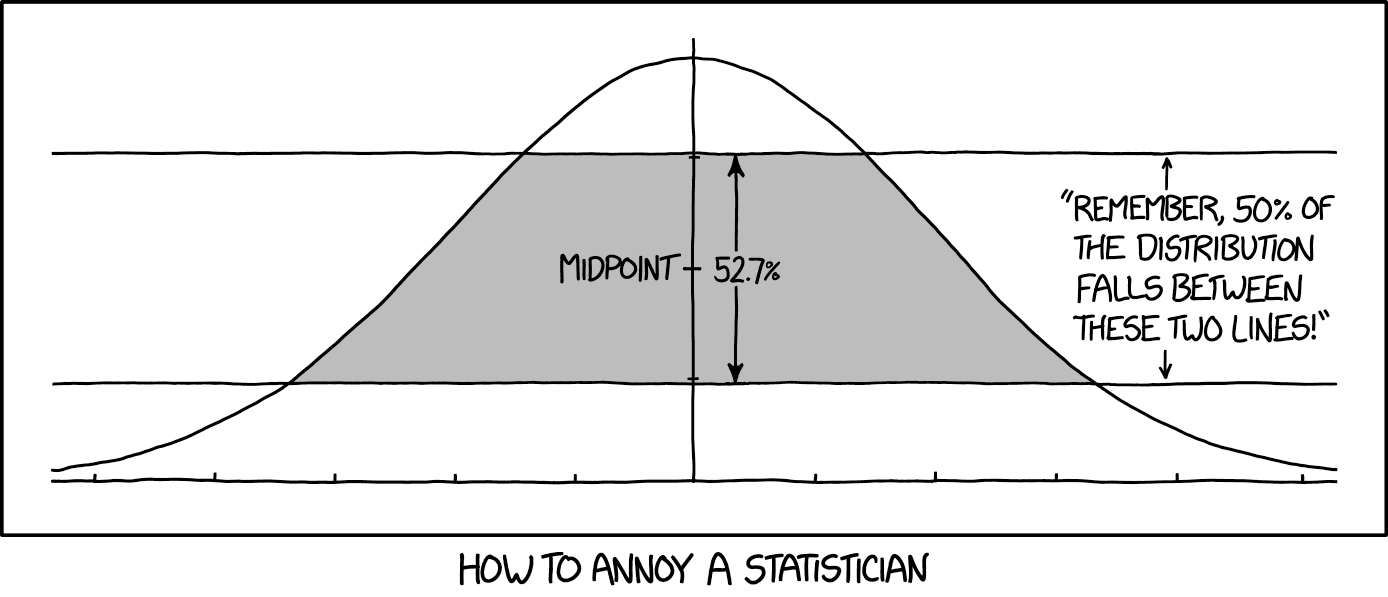
\includegraphics[width=\textwidth]{bilder/normal_distribution_2x.png}
    \caption*{It's the NORMAL distribution, not the TANGENT distribution.}
\end{figure*}
